\section{Exact Oracles in Directed Planar Graphs}\label{exactPlanar}

Previous works have given exact distance oracles for directed planar graphs of size
$O(n^{5/3})$ with query time $O(\lg n)$ \cite{cohen2017fast}. This was improved recently
to use $O(n^{3/2})$ space \cite{gawrychowski2017better}. In the general case, we have
bounds that depend on the number of vertices $n$. But in the vertex-labeled case, we can
sometimes win space or obtain better query times by depending on the number of labels $\ell$.

\subsection{A distance oracle depending on $\ell$}
We cannot directly adapt the approach used in \cite{cohen2017fast} and \cite{gawrychowski2017better} to work
for the vertex-labeled case as it requires us to know the "target" vertex. However,
depending on $\ell$, we can use the $r$-division alone to show the following:
\begin{thm}\label{thm1}
  There is a distance oracle with space $O(n\ell^{2/3)})$, query time $O(\ell^{1/3})$ and
  preprocessing time $O(n^2/\ell^{1/3})$.
\end{thm}
\textit{Data structure}. Given a directed graph $G$, with nonnegative edge lengths and a number of labels $\ell$, we
construct an $r$-division. Each region $R$ then has at most $r$ nodes and $O(\sqrt{r})$
boundary nodes. For each boundary node $u$, we store the shortest distance $d(u,\lambda)$
for all $\lambda \in L$ in a hash table. For all nodes inside $R$, we store the shortest
distance to all
boundary nodes as well as the distance to all labels present in $R$ in a hash table. \\
\\
\textit{Query}. Given the query $Q(v, \lambda)$, if $v$ is a boundary node, we can look
up the distance in the hash table for $v$. If $v$ is not a boundary node, look up the
distances $\delta(u,v)+\delta(u,\lambda)$ for all boundary nodes $u$ and the distance
$\delta(v,\lambda)$ stored in the hash table for $v$ and return the minimum.

\subsubsection{Analysis}
The $r$-division can be constructed in $O(n)$ time \cite{klein2013structured}. We then
construct a dense distance graph, that is, we construct the graph where each edge $uv\in
E$ has weight equal to $\delta(u,v)$ and $u$ and $v$ are both boundary nodes. We use
Klein's multiple source shortest path algorithm \cite{klein2005multiple} to compute DDG's
for each region of an $r$-division. For each region $R$ with $r$ nodes, we use $O(r\lg
r)$ preprocessing to compute distances $\delta(u,v)$ in $O(\lg r)$ time where either $u$
or $v$ is a boundary node. Since each region has $O(\sqrt{r})$ boundary nodes and $O(1)$
holes, we can compute all distances in $O(r\lg r)$ time. Since there are $O(n/r)$
regions, this yields a total running time of $O(nr\lg r/r)=O(n\lg r)$ to construct the
dense distance graph. We need to store distances from all boundary nodes to (potentially)
all other nodes in the graph. Henzinger et al. \cite{henzinger1997faster} gave a $O(n)$
time algorithm for single source shortest path in planar graphs. Using this for all
boundary nodes takes $O(n^2/\sqrt{r})$. To compute distances in the interior of each
region, we use Fredman and Tarjan's version of Djikstra's algorithm using Fibonacci heaps
\cite{fredman1987fibonacci}. This requires $O(n\lg n + m)$ time for each node. Each
region has $r$ vertices, the dense distance graph for the boundary nodes in the region has
$O(r)$ edges and the interior is a planar graph, so it has $O(r)$ edges as well. Using
this implementation for each node gives us a total running time of $O(r(r\lg r + r))=O(r^2\lg
r)$. The total preprocessing thus requires $O(n^2/\sqrt{r}+r^2\lg r)$ time. \\
\\
For each boundary node, we store the distance to all labels. The $r$-division gives us
$O(n/r)$ regions and ensures we
get $O(\sqrt{r})$ boundary nodes, so this yields
$O(\frac{n}{r}\sqrt{r}\ell)=O(\frac{n}{\sqrt{r}}\ell)$ space. For all other nodes, we
store the distances to all boundary nodes and to all labels within that region. This
gives us $O(nr)$ space as we can potentially store the distances to all vertices in a
region $R$. This gives us a total of $O(\frac{n}{\sqrt{r}}\ell+nr)$ space. \\
\\
The query $Q(u,\lambda)$ for a boundary node $u$ can be looked up in its hash table in
$O(1)$ time. For the query $Q(v,\lambda)$ for a vertex $v$ not on the boundary, we have
to find the minimum distance to $\lambda$ between all boundary nodes even if it exists in
that region as we are not guaranteed that the closest $\lambda$-labaled node is in the
region of $v$. Thus we have a query time of $O(\sqrt{r})$. \\
\\
This gives us a simple trade-off, since we can pick $r$ to be sufficiently small to
achieve constant query time, but this would give $O(n\ell)$ space. However, picking
$r=\ell^{2/3}$ and for $n$ sufficiently large, gives us $O(n^2/\ell^{1/3})$ preprocessing time, $O(n\ell^{2/3})$ space and query time $O(\ell^{1/3})$. This gives us Theorem $\ref{thm1}$.

\subsubsection{Recursion}
We can improve the trade-off slightly if we construct the $r$-division recursively. This will
yield space:
\begin{align*}
  \sum_{i=1}^{lg_{n/r}(n)} \left(\frac{n}{r}\right)^i
  \sqrt{r\left(\frac{r}{n}\right)^{i-1}} \min
  \left\{\ell,\left(n-r\right)\left(\frac{r}{n}\right)^{i-1}\right\}
\end{align*}
TODO: Not really worth it with recursion?

\subsection{A distance oracle with better query times}\label{oracle2}
We now present a distance oracle which is actually multiple data structures that perform
well depending on $\ell$ and the number of each $\lambda\in L$. We will refer to the
number of a given label by saying the \textit{size} of that label. Under the assumption
that $G$ does not have $\omega(\sqrt{n})$ labels of polynomial size, we can show the
following:
\begin{thm}\label{thm2}
  There is a distance oracle with space $O(n^{3/2})$, query time $O(\text{polylog}(n))$ and
  preprocessing time $O(n^2)$.
\end{thm}

\subsubsection{The data structure}
Given the directed graph $G$ and a number of labels $\ell$ with
$\varepsilon_1 = O(\sqrt{n})$ and $\varepsilon_2=O(\text{polylog}(n))$, we divide our
data structure into the following two cases: \\
\\
\textbf{Case 1:} If $\ell\in [1, \varepsilon_1]$, simply store the matrix of all shortest paths for all nodes to all
labels in the graph. \\
\\
\textbf{Case 2:} If $\ell\in (\varepsilon_1, n]$ and there are $\varepsilon_1$ number of labels that have
polynomial size, we employ two different strategies. For labels of size polynomial, we store the
shortest path from every vertex to those labels in a hash table. Additionally, for each
label, we store the size of that label. Otherwise, for labels that have size $\varepsilon_2$, we
use an approach similar to that described in \cite{cohen2017fast} and \cite{gawrychowski2017better}. \\
\\
The processing stage consists of finding a cycle separator of a planar graph
$G=(V,E)$ using a Jordan curve. This split the graph into two pieces $P=(V_P, E_P)$ and
$Q=(V_Q, E_Q)$. Using the separators recursively, we can compute a decomposition of $G$,
where each region has a constant number of holes. For all regions $R=(V_R, E_R)$ at some
step in the decomposition, we store a shortest path tree in that region, denoted $T_s$,
for all boundary nodes $s\in S$ in $R$. We also store all distances $\delta(s,u)$ and
$\delta(u,s)$ in the entire graph $G$. Whenever we separate a region into two pieces $P$
and $Q$, then for each hole $h\in P$ and node $u\in Q$, we store additevely weighted
Voronoi diagram $VD(S_h, w)$, where $S_h$ is the set of boundary nodes of $h$ and $w$ are
the distances from $u$ to all sites $s\in S_h$. TODO: Point location in Voronoi diagrams. These diagrams are also computed with $P$
and $Q$ interchanged. Figure \ref{vd1} illustrates the situation.

\begin{figure}[h!]
  \centering
  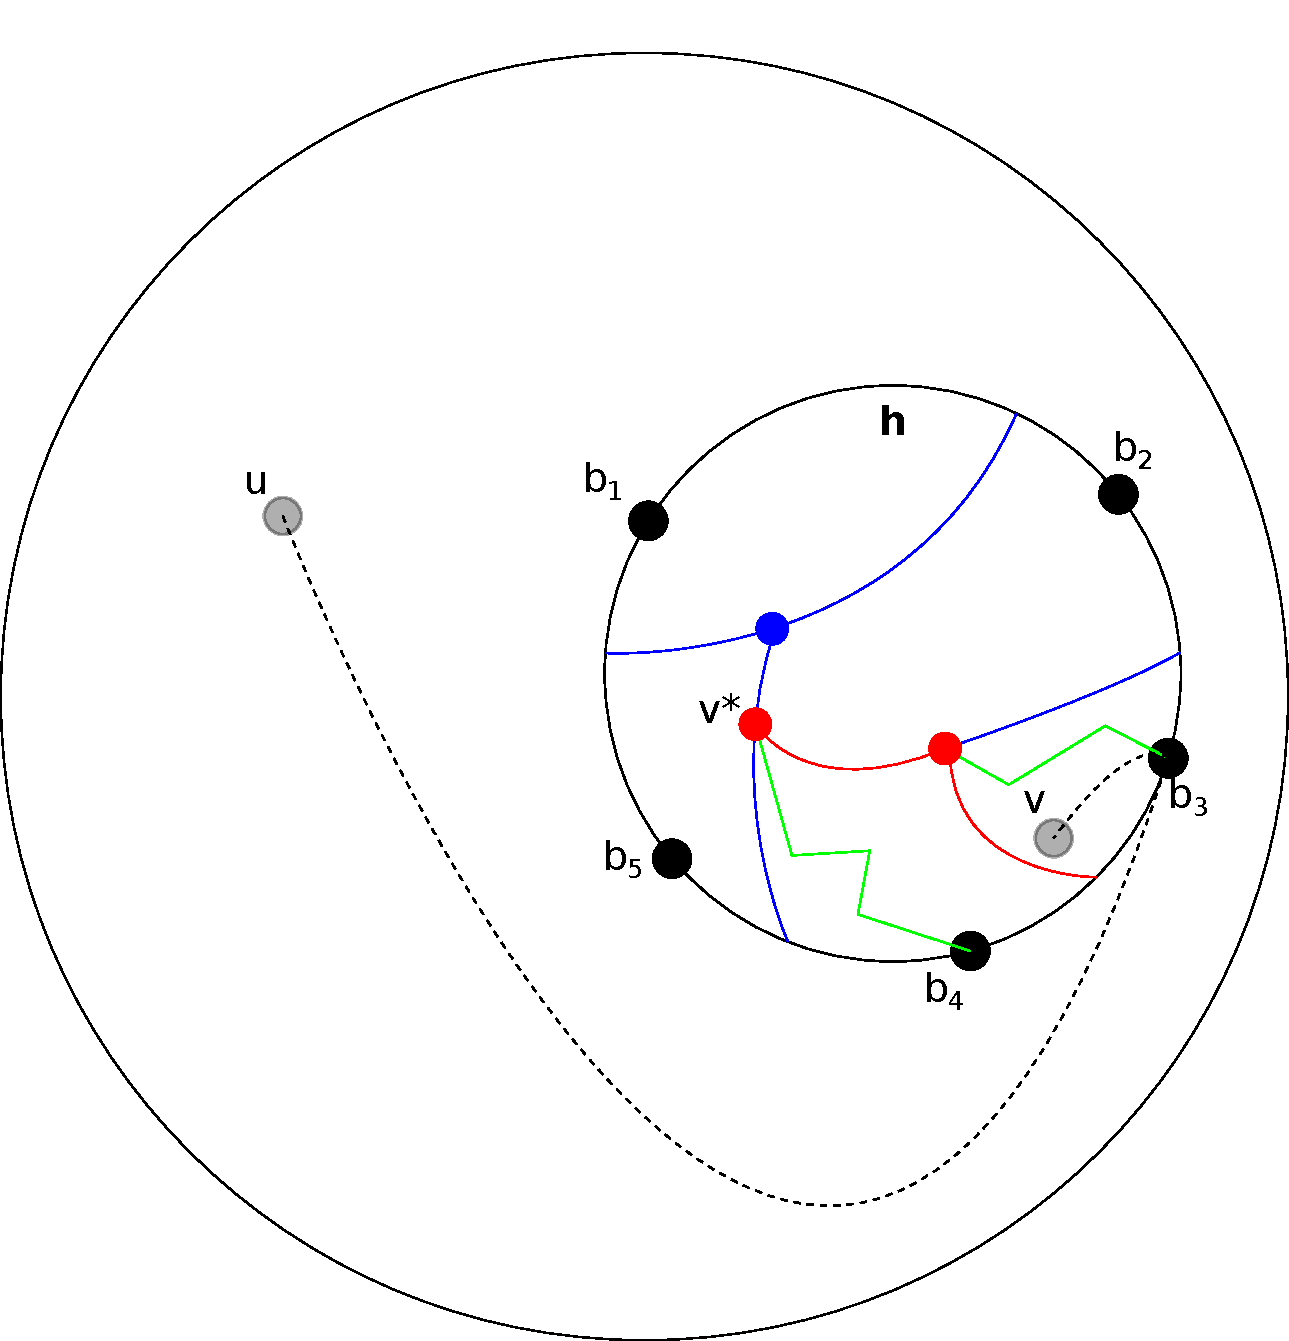
\includegraphics[width=0.66\textwidth]{figs/vd1.pdf}
  \caption{Illustration of stored information in the preprocessing stage.}
    \label{vd1}
\end{figure}



 \begin{itemize}
  \item Recursive decomposition using Jordan curves.
  \item Voronoi diagrams
  \item Distances stored
  \item Point location approach
\end{itemize}
\noindent \\
\textit{Query}. Depending on the case that $G$ falls under, we do the following for the
query $Q(v, \lambda)$: \\
\\
\textbf{Case 1:} Look up the distance in the hash table stored for $v$. \\
\textbf{Case 2:} The query works in the same manner as described in section
\ref{cohenplanar}, however, we do not the target vertex. Therefore, we have to run over
all vertices with label $\lambda$ and return the minimal distance. \\
\textbf{Case 3:} First we look up the size of $\lambda$ in the hash table. If the size of
$\lambda$ is $\varepsilon_2$, we do the same as in case 2. If the size of $\lambda$ is
$\omega(\text{polylog}(n))$, we look up the distance stored in the hash table for $v$.

\subsubsection{Analysis}
Henzinger et al. showed that single source shortest paths can be computed in $O(n)$ time
\cite{henzinger1997faster} assuming non-negative edge lengths. Preprocessing can thus be done in $O(n^2)$. TODO: better. \\
\\
In case 1, we store $\ell$ distances for each vertex $v$. Since $\ell=O(\sqrt{n})$, this
yields space $O(n^{3/2})$. \\
In case 2, space follows directly from \cite{gawrychowski2017better} as the construction
is identical, which is $O(n^{3/2})$. \\
In case 3, we perform the same construction as in \cite{gawrychowski2017better} requiring
in $O(n^{3/2})$ space. Additionally, since we assumed that there are no more that
$O(\sqrt{n})$ labels of size $\omega(\text{polylog}(n))$, the hash table storing the
distances to these labels cannot require more than $O(n^{3/2})$ space. The hash table
storing the size of all labels require $O(\ell)$ space, so the total space
in this case (and in any other case) is $O(n^{3/2})$.\\
\\
In case 1, we look up the distance in the hash table in $O(1)$ time.\\
In case 2, all labels have size $O(\text{polylog}(n))$. Since the point location desribed
in \cite{gawrychowski2017better} takes $O(\lg n)$ and we need to do at most
$O(\text{polylog}(n))$ of these point location, the total query time is
$O(\text{polylog}(n))$. \\
In case 3, we do a lookup in the hash table storing the sizes of each $\lambda\in L$ in
$O(1)$ time. Depending on the result, we either do the same thing as in case 1 or case 2,
thus we have a query time of $O(\text{polylog}(n))$. \\
\\
This gives us the distance oracle given in Theorem \ref{thm2}. \\
\\
TODO: Fix the gap ($\omega(\sqrt{n})$ labels with $\omega(\text{polylog}(n))$ size).
